\documentclass{article}
\renewcommand\refname{Referencias}
\renewcommand\contentsname{\'Indice de Conten\'ido}
\usepackage{graphicx}
\graphicspath{{EJ1}{EJ2}{EJ3}{EJ4}}
\usepackage{caption}
\usepackage{subcaption}
\usepackage{float}

\title{\textsc{Inteligencia Artificial\\Trabajo Pr\'actico 3:\\B\'usquedas - Heur\'istica}}
\author{Ulises C. Ramirez}
\date{17 de Septiembre, 2018}

\begin{document}
\maketitle
\pagenumbering{gobble}
\newpage
\section*{Versionado}
Para el corriente documento se est\'a llevando un versionado a fin de mantener un respaldo del trabajo y adem\'as proveer a la c\'atedra o a cualquier interesado la posibilidad de leer el material en la \'ultima versi\'on disponible.\\

\begin{center}
  \textsc{Repositorio}: \textit{https://github.com/ulisescolina/UC-IA/tree/master/TP/Busquedas}
\end{center}


\hfill--\textsc{Ulises}
\tableofcontents
\pagenumbering{gobble}
\newpage

% === Inicio del Cuerpo del Documento === %
\pagenumbering{arabic}
\section{Ejercicio 1}
\label{sec:ej1}
\textsc{Consigna}: \textbf{Trace como opera la b\'usqueda A* aplicada al problema de alcanzar Bucarest desde Lugoj utilizando la heur\'istica distancia en l\'inea recta. Es decir, muestre la secuencia de nodos que considerará el algoritmo y los valores de f, g, y h para cada nodo.}\\

A continuaci\'on se proveeran las im\'agenes para el paso a paso del algoritmo A* para alcanzar Bucharest en el mapa que provee la diapositiva.

\begin{figure}[H]
  \centering
  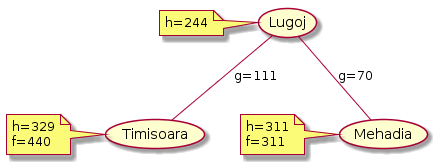
\includegraphics[width=.4\linewidth]{EJ2/As.png}
  \caption{Primer paso para el algoritmo A*}
\end{figure}

\begin{figure}[H]
  \centering
  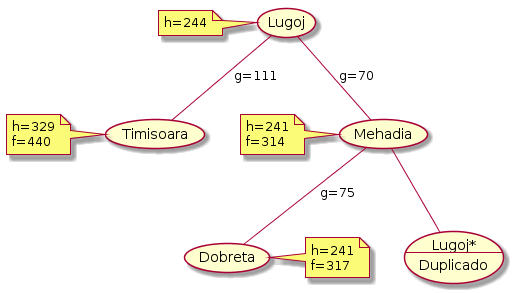
\includegraphics[width=.4\linewidth]{EJ2/As_001.png}
  \caption{Segundo paso para el algoritmo A*}
\end{figure}

\begin{figure}[H]
  \centering
  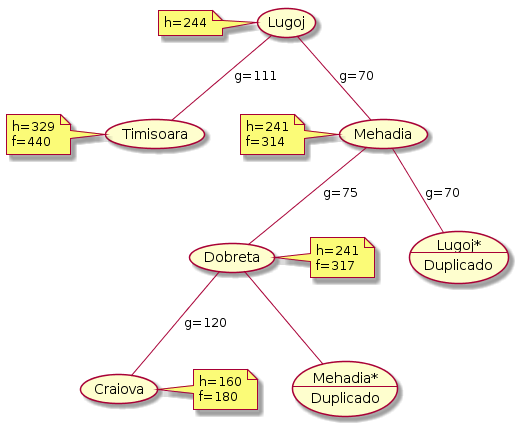
\includegraphics[width=.4\linewidth]{EJ2/As_002.png}
  \caption{Tercer paso para el algoritmo A*}
\end{figure}

\begin{figure}[H]
  \centering
  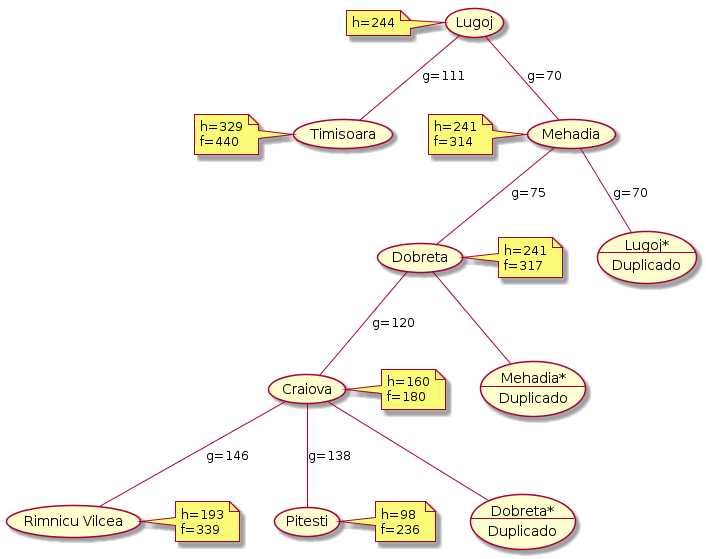
\includegraphics[width=.4\linewidth]{EJ2/As_003.png}
  \caption{Cuarto paso para el algoritmo A*}
\end{figure}

\begin{figure}[H]
  \centering
  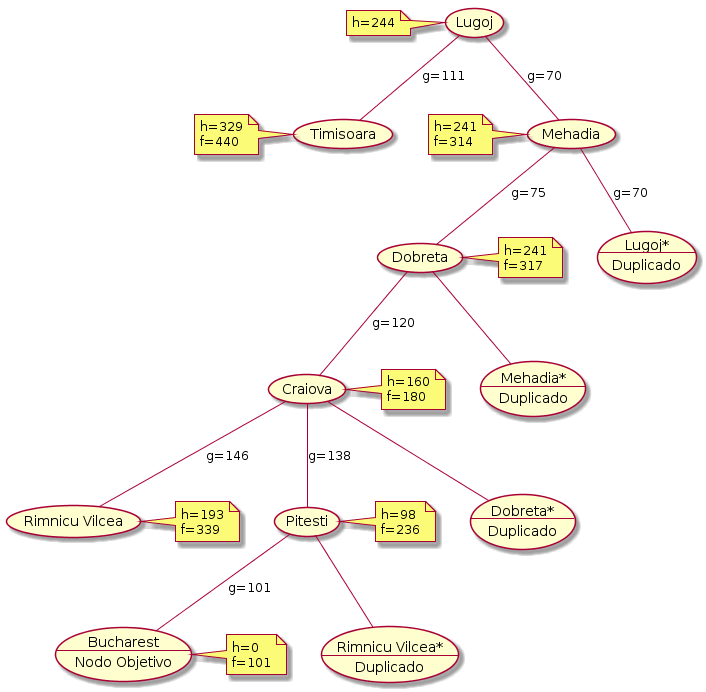
\includegraphics[width=.4\linewidth]{EJ2/As_004.png}
  \caption{Quinto paso para el algoritmo A*}
\end{figure}

\section{Ejercicio 2}
\textsc{Consigna}: \textbf{dado el grafo descrito en la \texttt{Figura \ref{gra:g1}} describa la expansi\'on de nodos, primero en profundidad luego primero en amplitud considerando a ``A'' como nodo inicial y a ``K'' como nodo objetivo.
\begin{figure}[H]
  \centering
  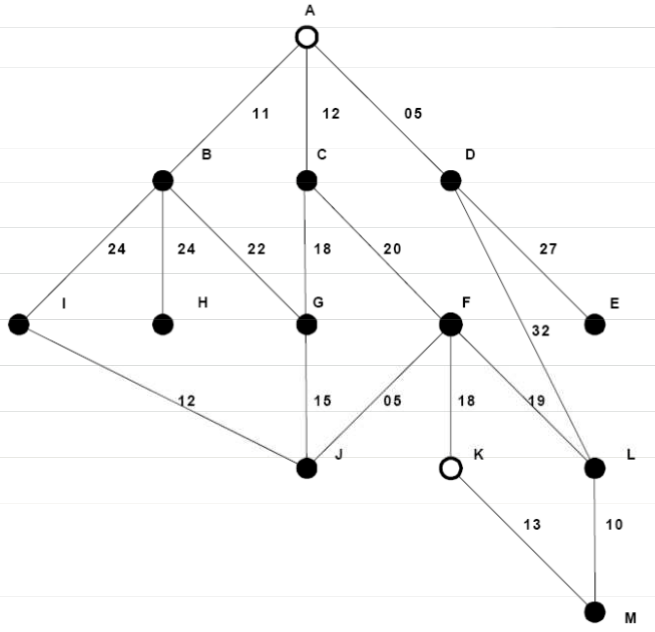
\includegraphics[width=.4\linewidth]{diap52.png}
  \caption{Ejercicio Diapositiva 52}
  \label{gra:g1}
\end{figure}
}

\subsection{Primero en Profundidad}

\begin{figure}[H]
  \centering
  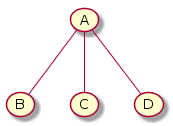
\includegraphics[width=.4\linewidth]{EJ3/profundidad.png}
  \caption{Primer paso para el Algoritmo Primero en Profundidad}
  \label{gr:g2}
\end{figure}

\begin{figure}[H]
  \centering
  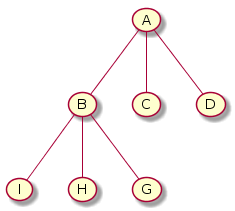
\includegraphics[width=.4\linewidth]{EJ3/profundidad_001.png}
  \caption{Segundo paso para el Algoritmo Primero en Profundidad}
  \label{gr:g3}
\end{figure}

\begin{figure}[H]
  \centering
  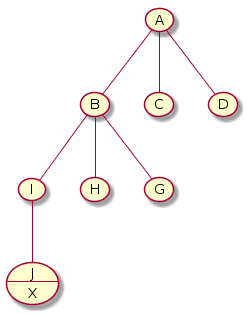
\includegraphics[width=.4\linewidth]{EJ3/profundidad_002.png}
  \caption{Tercer paso para el Algoritmo Primero en Profundidad}
  \label{gr:g4}
\end{figure}
\begin{figure}[H]
  \centering
  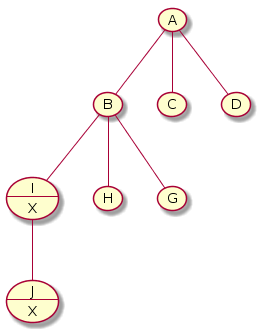
\includegraphics[width=.4\linewidth]{EJ3/profundidad_003.png}
  \caption{Cuarto paso para el Algoritmo Primero en Profundidad}
  \label{gr:g5}
\end{figure}
\begin{figure}[H]
  \centering
  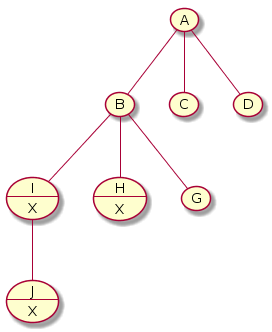
\includegraphics[width=.4\linewidth]{EJ3/profundidad_004.png}
  \caption{Quinto paso para el Algoritmo Primero en Profundidad}
  \label{gr:g6}
\end{figure}
\begin{figure}[H]
  \centering
  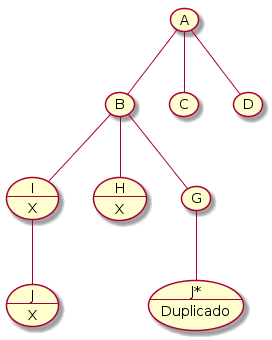
\includegraphics[width=.4\linewidth]{EJ3/profundidad_005.png}
  \caption{Sexto paso para el Algoritmo Primero en Profundidad}
  \label{gr:g7}
\end{figure}
\begin{figure}[H]
  \centering
  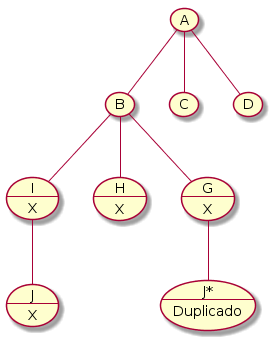
\includegraphics[width=.4\linewidth]{EJ3/profundidad_006.png}
  \caption{S\'eptimo paso para el Algoritmo Primero en Profundidad}
  \label{gr:g8}
\end{figure}
\begin{figure}[H]
  \centering
  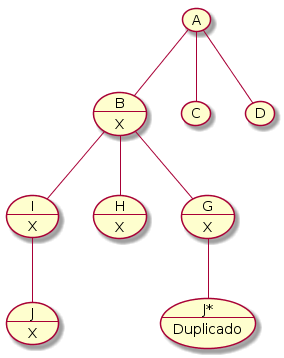
\includegraphics[width=.4\linewidth]{EJ3/profundidad_007.png}
  \caption{Octavo paso para el Algoritmo Primero en Profundidad}
  \label{gr:g9}
\end{figure}
\begin{figure}[H]
  \centering
  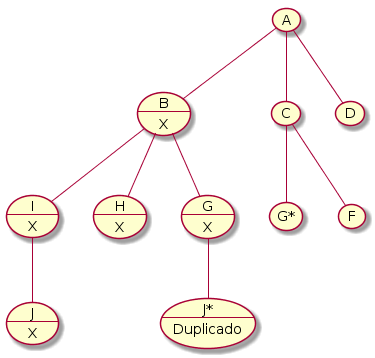
\includegraphics[width=.4\linewidth]{EJ3/profundidad_008.png}
  \caption{Noveno paso para el Algoritmo Primero en Profundidad}
  \label{gr:g10}
\end{figure}
\begin{figure}[H]
  \centering
  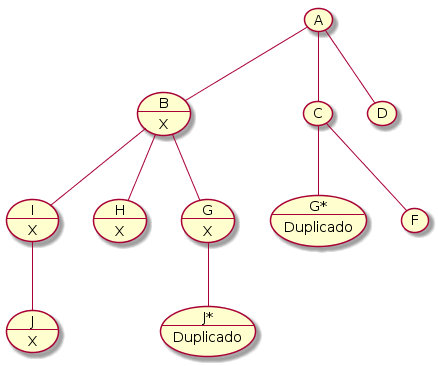
\includegraphics[width=.4\linewidth]{EJ3/profundidad_009.png}
  \caption{D\'ecimo paso para el Algoritmo Primero en Profundidad}
  \label{gr:g11}
\end{figure}
\begin{figure}[H]
  \centering
  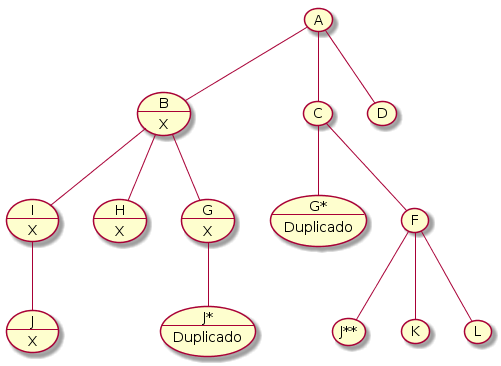
\includegraphics[width=.4\linewidth]{EJ3/profundidad_010.png}
  \caption{D\'ecimo primer paso para el Algoritmo Primero en Profundidad}
  \label{gr:g12}
\end{figure}
\begin{figure}[H]
  \centering
  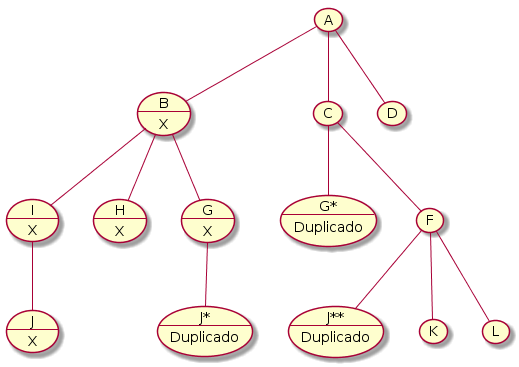
\includegraphics[width=.4\linewidth]{EJ3/profundidad_011.png}
  \caption{D\'ecimo segundo paso para el Algoritmo Primero en Profundidad}
  \label{gr:g13}
\end{figure}

\subsection{Primero en Amplitud}

\begin{figure}[H]
  \centering
  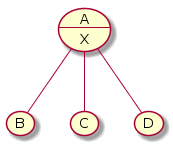
\includegraphics[width=.4\linewidth]{EJ4/ej4.png}
  \caption{Primer paso para el Algoritmo Primero en Amplitud}
  \label{gr:g14}
\end{figure}

\begin{figure}[H]
  \centering
  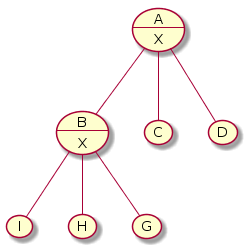
\includegraphics[width=.4\linewidth]{EJ4/ej4_001.png}
  \caption{Segundo paso para el Algoritmo Primero en Amplitud}
  \label{gr:g15}
\end{figure}

\begin{figure}[H]
  \centering
  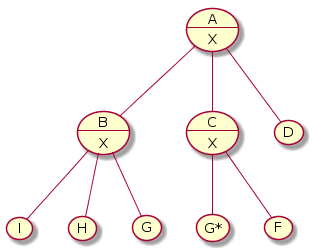
\includegraphics[width=.4\linewidth]{EJ4/ej4_002.png}
  \caption{Tercer paso para el Algoritmo Primero en Amplitud}
  \label{gr:g16}
\end{figure}

\begin{figure}[H]
  \centering
  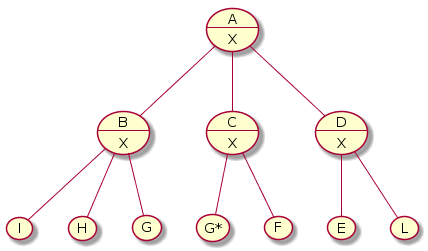
\includegraphics[width=.4\linewidth]{EJ4/ej4_003.png}
  \caption{Cuarto paso para el Algoritmo Primero en Amplitud}
  \label{gr:g17}
\end{figure}

\begin{figure}[H]
  \centering
  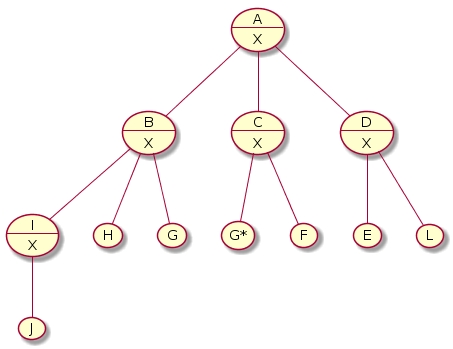
\includegraphics[width=.4\linewidth]{EJ4/ej4_004.png}
  \caption{Quinto paso para el Algoritmo Primero en Amplitud}
  \label{gr:g18}
\end{figure}

\begin{figure}[H]
  \centering
  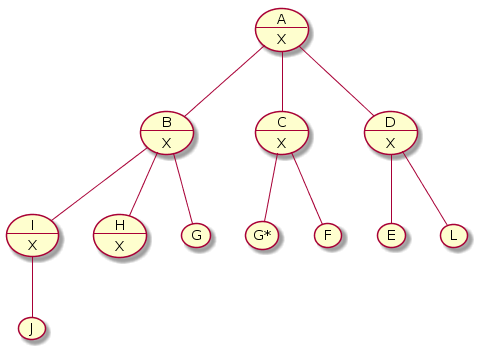
\includegraphics[width=.4\linewidth]{EJ4/ej4_005.png}
  \caption{Sexto paso para el Algoritmo Primero en Amplitud}
  \label{gr:g19}
\end{figure}

\begin{figure}[H]
  \centering
  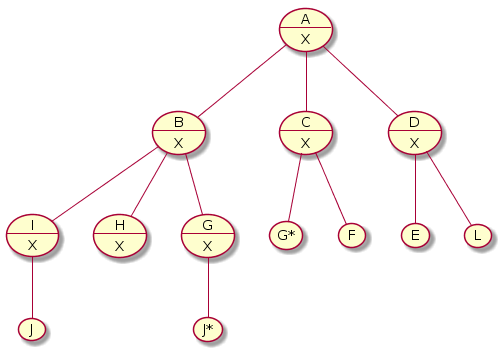
\includegraphics[width=.4\linewidth]{EJ4/ej4_006.png}
  \caption{S\'eptimo paso para el Algoritmo Primero en Amplitud}
  \label{gr:g20}
\end{figure}

\begin{figure}[H]
  \centering
  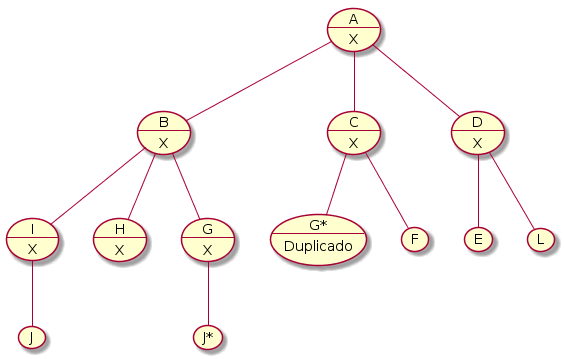
\includegraphics[width=.4\linewidth]{EJ4/ej4_007.png}
  \caption{Octavo paso para el Algoritmo Primero en Amplitud}
  \label{gr:g21}
\end{figure}

\begin{figure}[H]
  \centering
  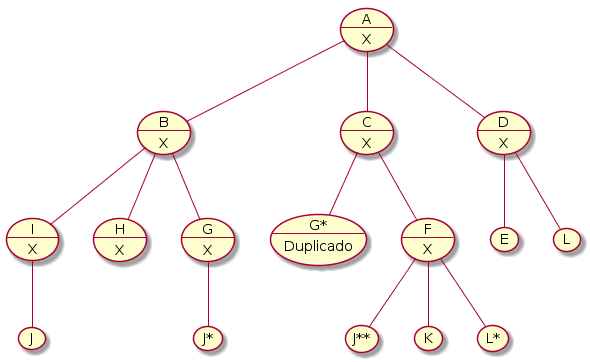
\includegraphics[width=.4\linewidth]{EJ4/ej4_008.png}
  \caption{Noveno paso para el Algoritmo Primero en Amplitud}
  \label{gr:g22}
\end{figure}

\begin{figure}[H]
  \centering
  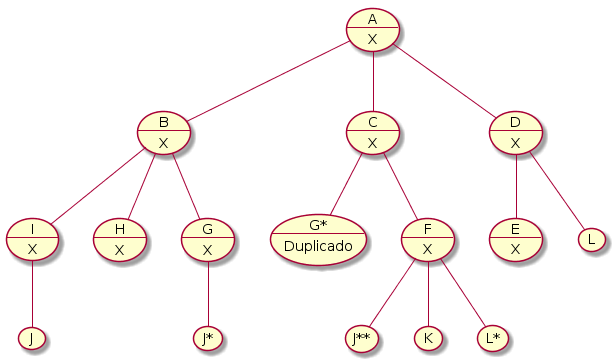
\includegraphics[width=.4\linewidth]{EJ4/ej4_009.png}
  \caption{D\'ecimo paso para el Algoritmo Primero en Amplitud}
  \label{gr:g23}
\end{figure}

\begin{figure}[H]
  \centering
  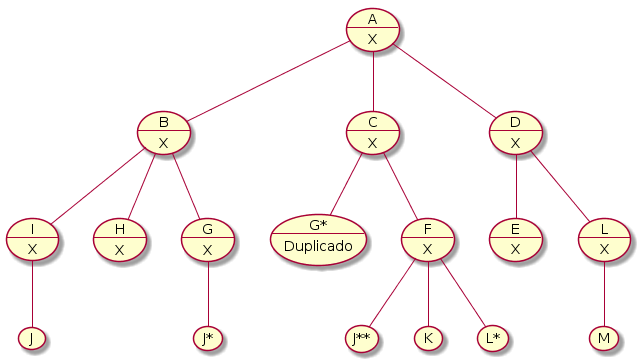
\includegraphics[width=.4\linewidth]{EJ4/ej4_010.png}
  \caption{D\'ecimo primer paso para el Algoritmo Primero en Amplitud}
  \label{gr:g24}
\end{figure}

\begin{figure}[H]
  \centering
  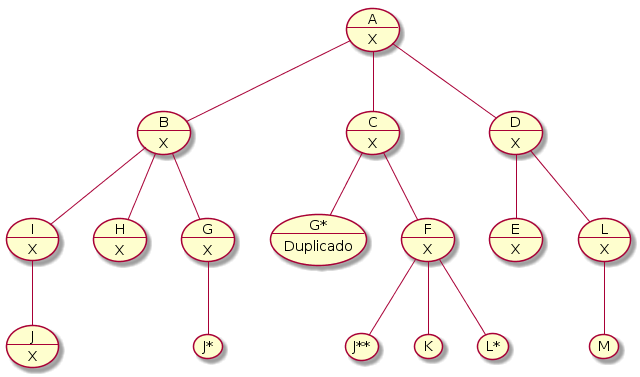
\includegraphics[width=.4\linewidth]{EJ4/ej4_011.png}
  \caption{D\'ecimo segundo paso para el Algoritmo Primero en Amplitud}
  \label{gr:g25}
\end{figure}

\begin{figure}[H]
  \centering
  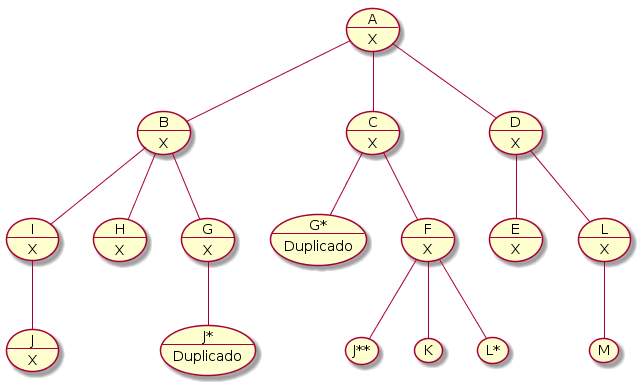
\includegraphics[width=.4\linewidth]{EJ4/ej4_012.png}
  \caption{D\'ecimo tercer para el Algoritmo Primero en Amplitud}
  \label{gr:g26}
\end{figure}

\begin{figure}[H]
  \centering
  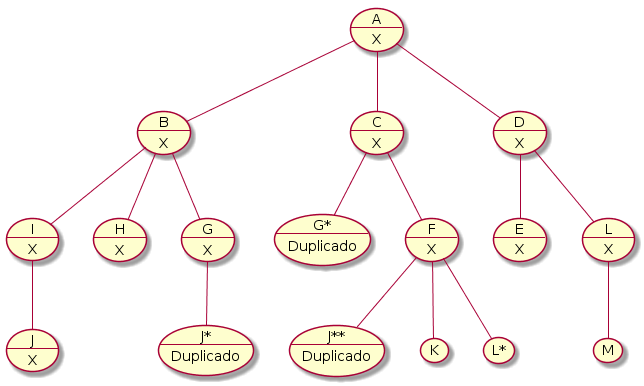
\includegraphics[width=.4\linewidth]{EJ4/ej4_013.png}
  \caption{D\'ecimo cuarto paso para el Algoritmo Primero en Amplitud}
  \label{gr:g27}
\end{figure}

\begin{figure}[H]
  \centering
  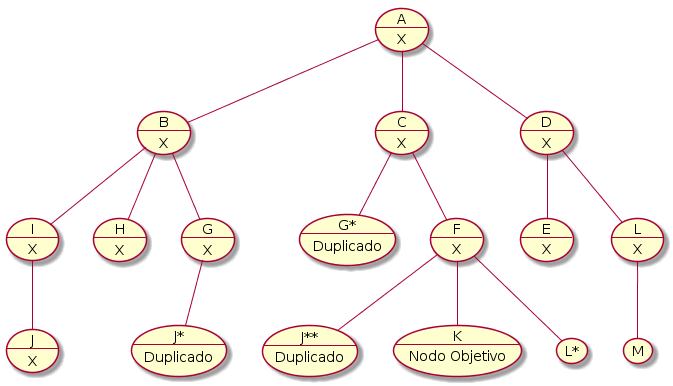
\includegraphics[width=.4\linewidth]{EJ4/ej4_014.png}
  \caption{D\'ecimo quinto paso para el Algoritmo Primero en Amplitud}
  \label{gr:g28}
\end{figure}
\end{document}
